\section{Link Layer}
\label{sec:link}

Two half-duplex stations form \emph{two directed links}, each governed
by its receiver --- only the receiver knows its own noise floor.  There
is no shared ``link mode'' to negotiate; each side requests what it can
hear.

\subsection{The Rate Ladder}

Thirteen operating points (mode $\times$ modulation $\times$ code
rate, dominated rungs removed) span \textbf{7.8--1059\,bit/s} over
\textbf{$-17.9\ldots+4.7$\,dB} (Table~\ref{tab:ladder}).  Every
sensitivity is measured, not derived
(\texttt{experiments/ladder\_sweep.py}, 48 packets/point, recalibrated
receiver; full PER curves in \texttt{results/ladder\_recal.json}).
Requests and grants are ladder indices carried in the link-control
word.  One quirk is documented: rung 1 (ROBUST BPSK 1/3) is dominated
by rung 2 (faster, equally sensitive) and is kept only for
ladder-index stability --- it is never selected.

\begin{table}[H]
    \centering
    \caption{The measured rate ladder (PER $\le 10\,\%$ sensitivities,
             recalibrated receiver, 6\,kHz-band SNR).}
    \label{tab:ladder}
    \small
    \begin{tabular}{@{}rlrr@{\hspace{2em}}rlrr@{}}
    \toprule
    \# & \textbf{mode/mod/FEC} & \textbf{bit/s} & \textbf{dB} &
    \# & \textbf{mode/mod/FEC} & \textbf{bit/s} & \textbf{dB} \\
    \midrule
    0 & EXTREME BPSK 1/3 & 7.8 & $-17.9$ & 7  & NORMAL QPSK 1/2  & 353  & $-5.3$ \\
    1 & ROBUST BPSK 1/3  & 31  & $-11.7$ & 8  & NORMAL QPSK 2/3  & 471  & $-3.8$ \\
    2 & ROBUST BPSK 1/2  & 46  & $-11.8$ & 9  & NORMAL QPSK 3/4  & 529  & $-2.2$ \\
    3 & ROBUST QPSK 1/3  & 62  & $-11.3$ & 10 & NORMAL QAM16 1/2 & 706  & $+0.7$ \\
    4 & NORMAL BPSK 1/3  & 118 & $-7.6$  & 11 & NORMAL QAM16 2/3 & 941  & $+2.6$ \\
    5 & NORMAL BPSK 1/2  & 176 & $-7.3$  & 12 & NORMAL QAM16 3/4 & 1059 & $+4.7$ \\
    6 & NORMAL QPSK 1/3  & 235 & $-7.0$  &    &                  &      &         \\
    \bottomrule
    \end{tabular}
\end{table}

\subsection{The Link-Control Word}

Every frame --- data, ACKs, everything --- piggybacks a 20-bit word in
\texttt{Data.reserved}:
\texttt{seq(2)\,|\,ack(2)\,|\,req\_rung(4)\,|\,snr\_report(4)\,|\,%
freq\_corr(5)\,|\,flags(3)}.  The SNR report uses 2\,dB steps
over codes 1--15 $= -22\ldots+6$\,dB; \textbf{code 0 means ``no
measurement''}, not $-24$\,dB, and the transmit-rung cap derived from
the peer's report is applied only when a report exists.  The
distinction was learned on the air (\S\ref{sec:cport_sentinel}): the
filtered-SNR getter returns a $-99$\,dB sentinel once every sample has
aged past 60\,s, and packing that into the wire's low rail made a
peer read a real $-24$\,dB and cap its rung to 0.  The
frequency-correction field carries $\pm 120$\,Hz in 8\,Hz steps
(\S\ref{sec:afc}).  The three flag bits are last-fragment, no-data
(ACK-only) and priority-stream, and their three ``impossible''
combinations are spent on the C stack's extensions: two on the burst
acknowledgment and burst data frames (\S\ref{sec:cport_proto}) and the
third, flags~7, on the capability record (\S\ref{sec:cport_caps}).

\subsection{Rate Adaptation: Three Feedback Paths}

Figure~\ref{fig:adaptation} shows the controller.  On the receive
side, per-frame SNR estimates pass through a fade-aware filter (the
second-lowest of recent measurements, age-windowed to 60\,s) before
driving the rung request: upshift requires the target rung's
sensitivity plus 2.5\,dB of held margin, downshift triggers below
1\,dB (the hysteresis band prevents ping-pong), and inbound
\emph{silence} decays the request and purges the measurement history
--- without the purge, stale pre-fade measurements resurrect a high
rung the moment one frame gets through.

\begin{figure}[H]
    \centering
    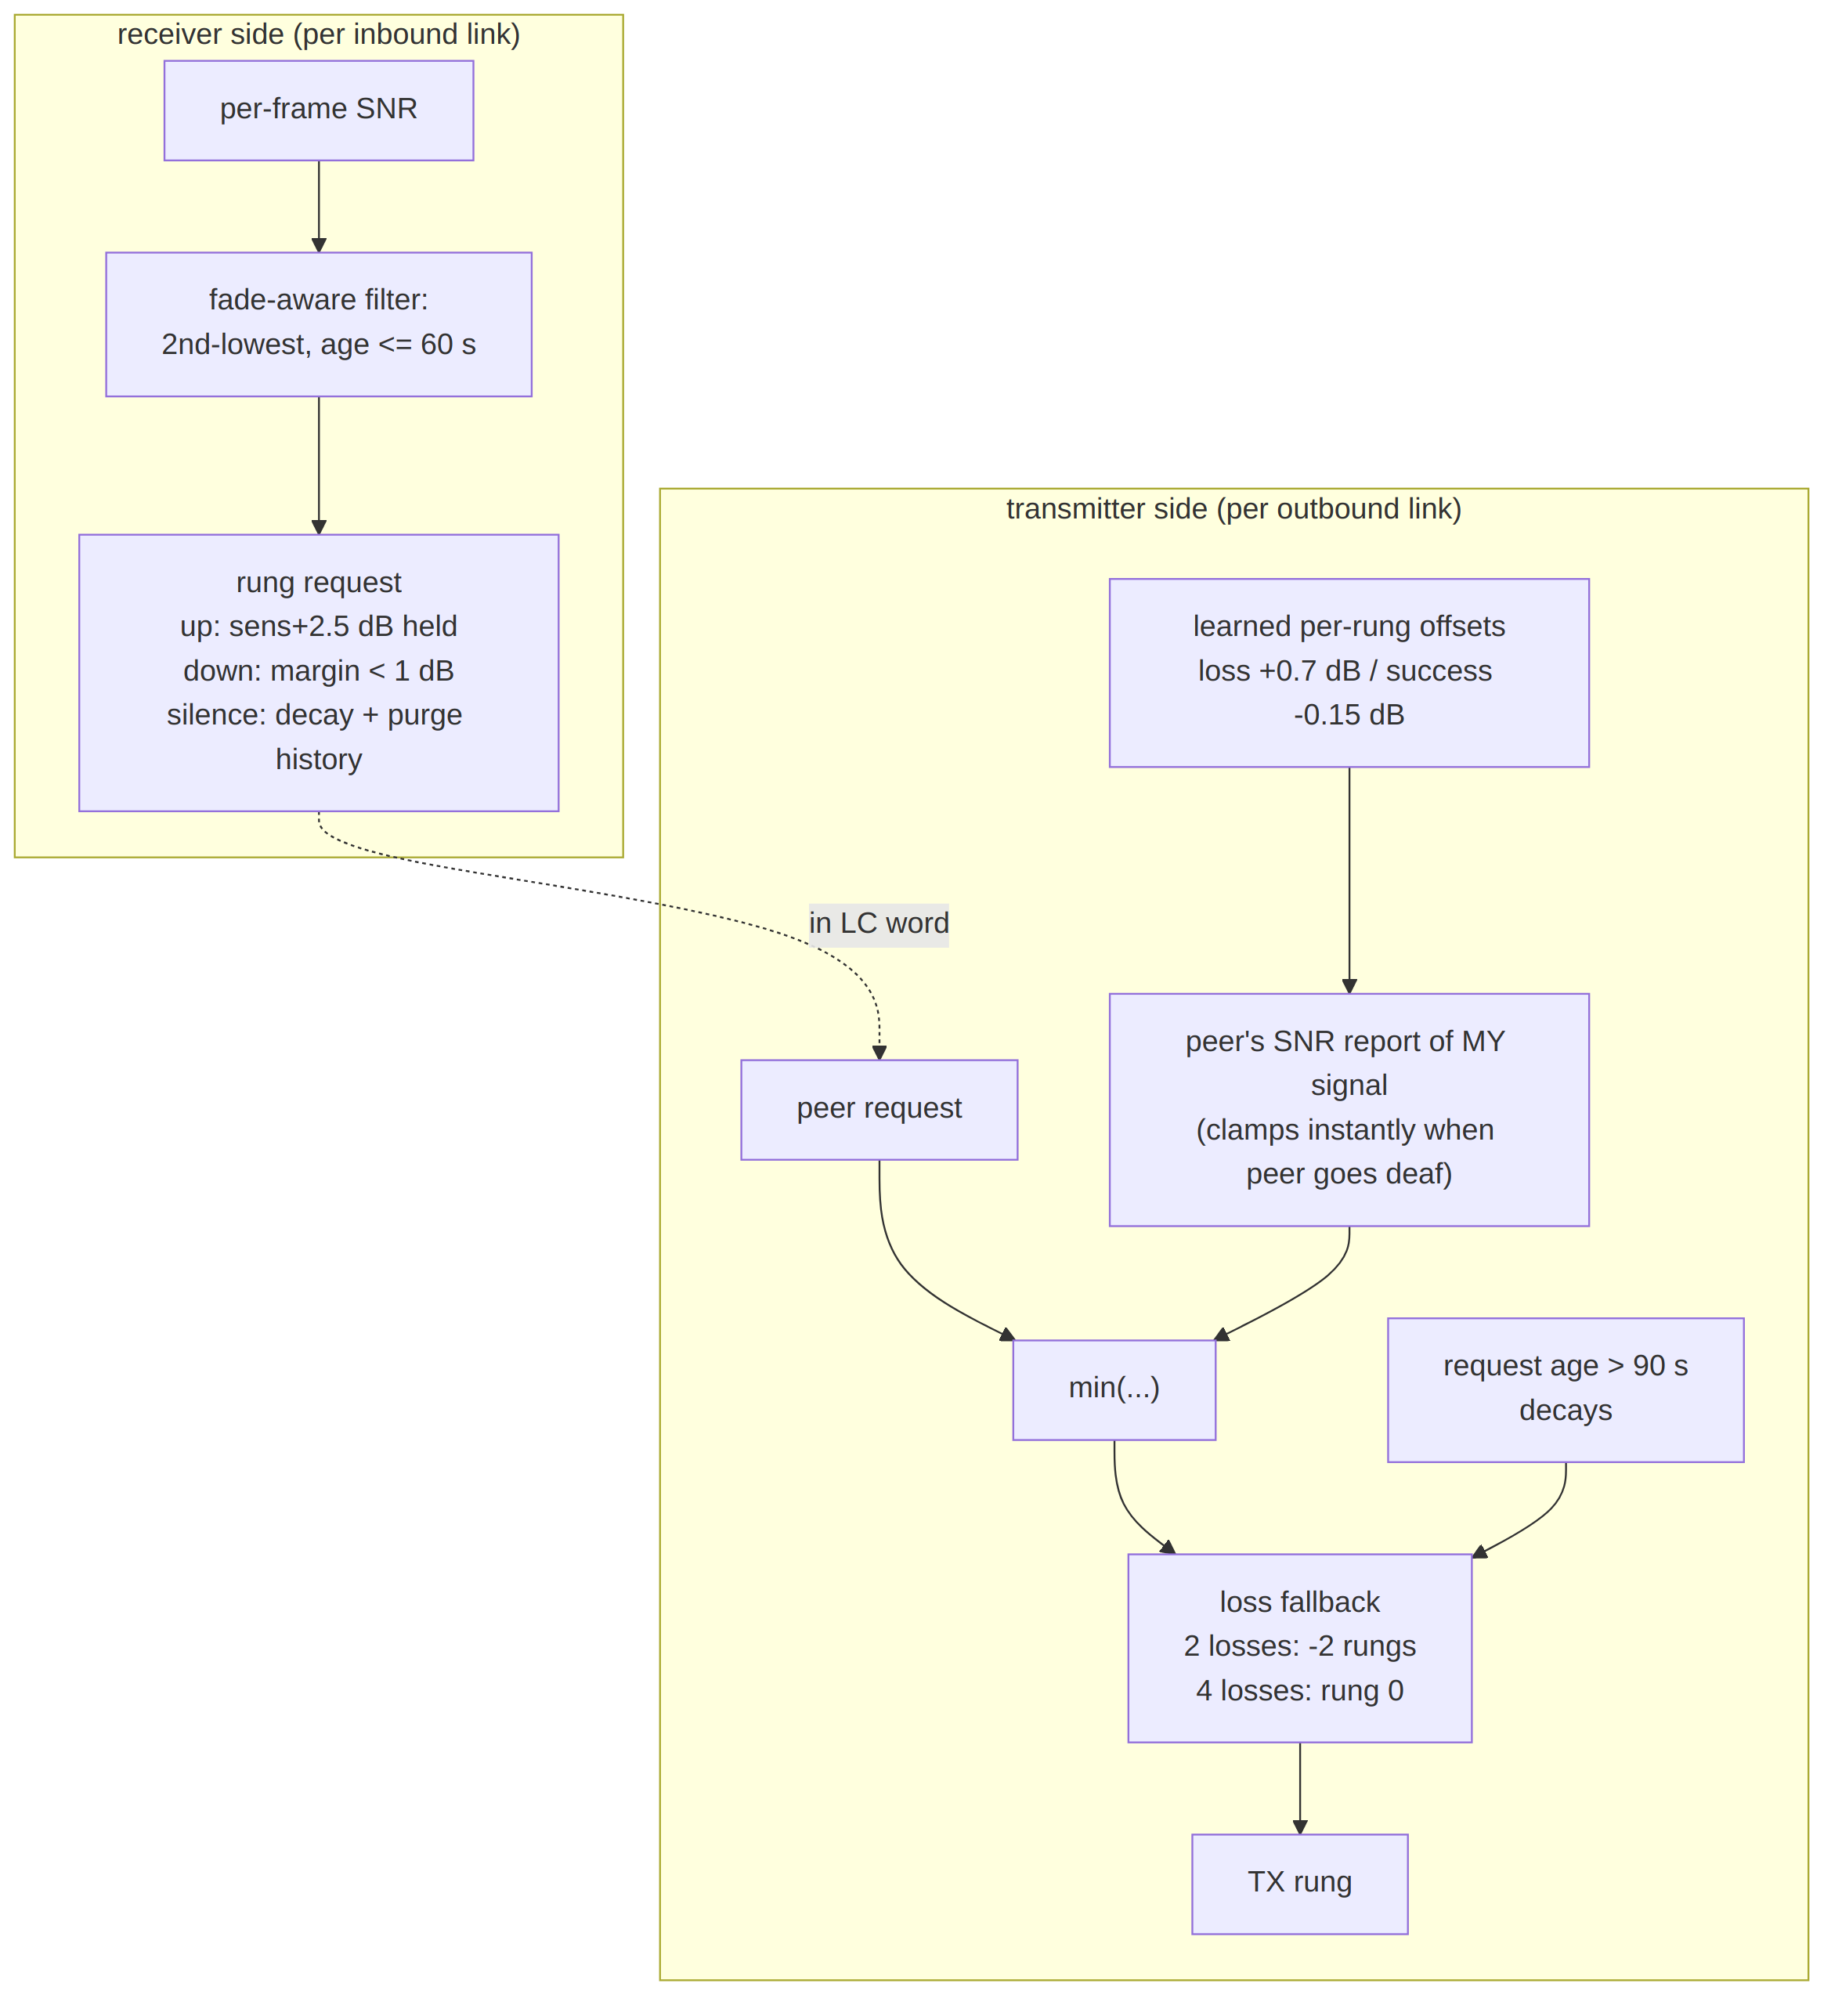
\includegraphics[width=\textwidth]{images/adaptation.png}
    \caption{Receiver-driven rate adaptation.  The three feedback paths
             have three different latencies: the peer's explicit
             request (one round trip), the peer's SNR report of
             \emph{your} signal (instant clamp when the peer goes
             deaf), and loss-driven fallback (no feedback at all).}
    \label{fig:adaptation}
\end{figure}

Figure~\ref{fig:rungseq} walks the same controller through one
session.  The three paths differ in what they need in order to act:
the peer's explicit request needs a round trip, the peer's SNR report
of \emph{our} signal clamps the cap as soon as any frame arrives, and
the loss fallback needs no feedback at all --- which is the only path
still available once the peer has gone silent.

\begin{figure}[H]
    \centering
    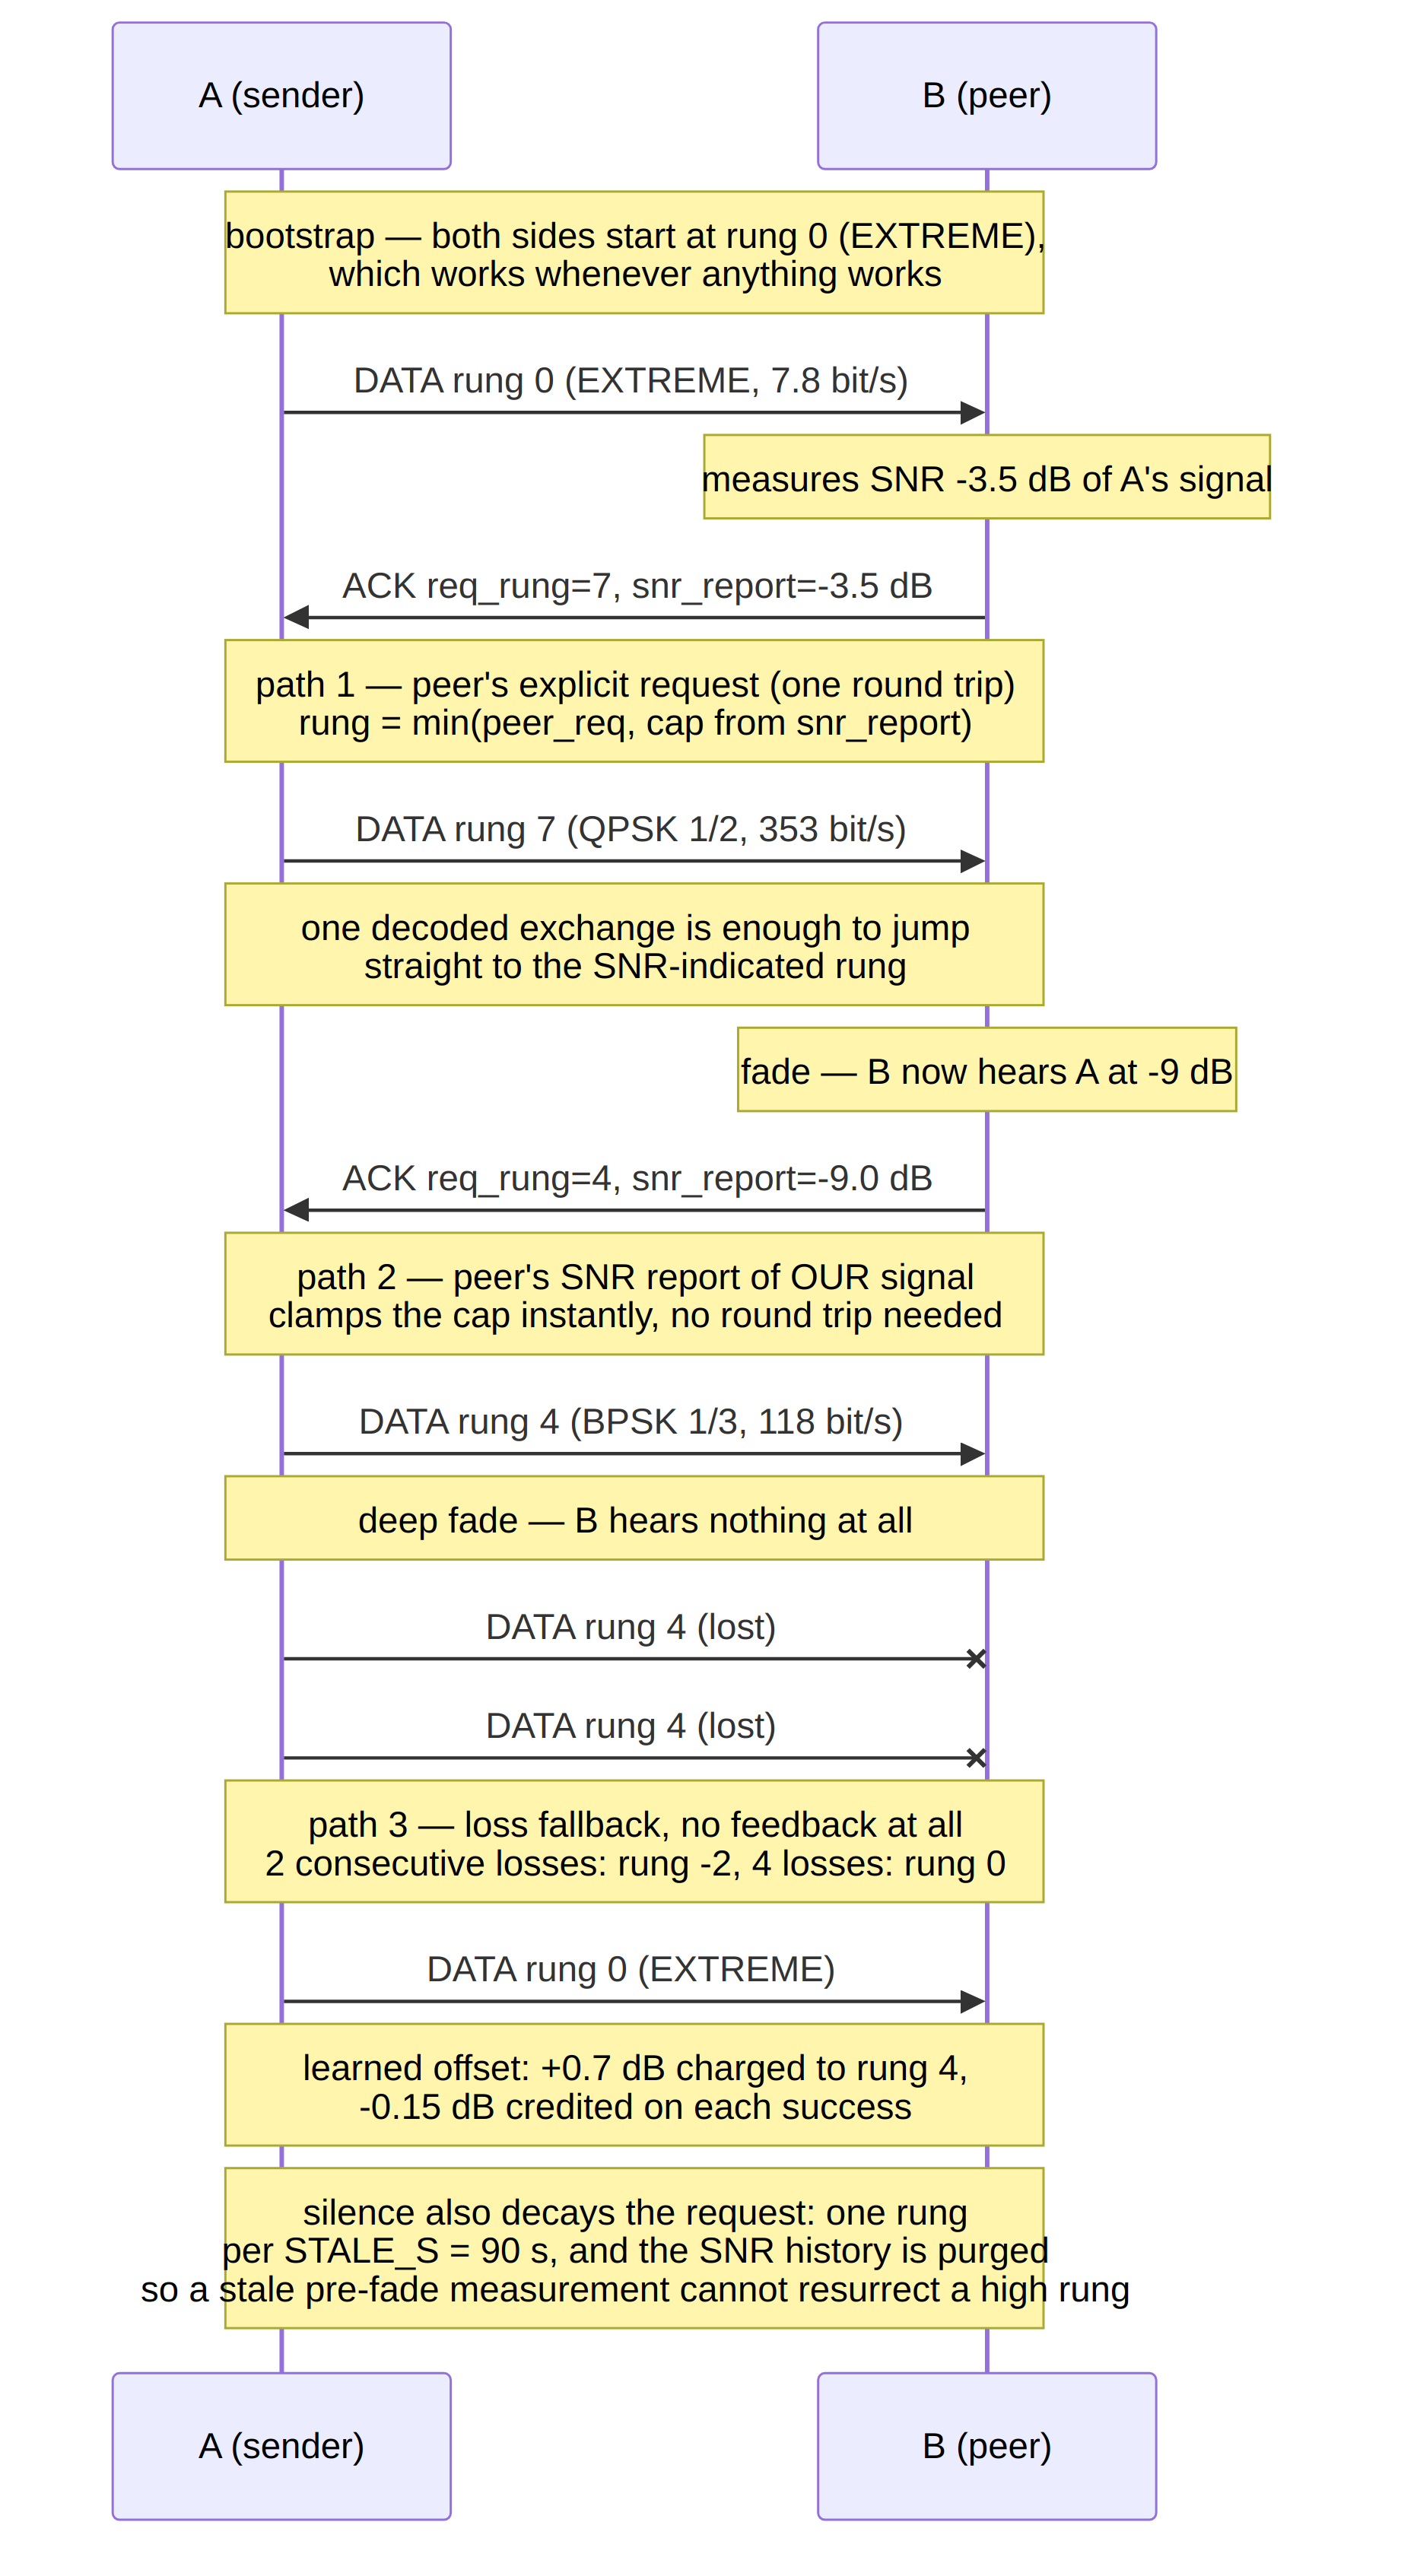
\includegraphics[width=0.80\textwidth]{images/rung_seq.png}
    \caption{Rung selection across modes: bootstrap at rung~0
             (EXTREME), the jump to the SNR-indicated rung after a
             single decoded exchange, a fade clamped by the peer's
             report, and the loss fallback when no feedback arrives at
             all.  Silence is not neutral --- it decays the request by
             one rung per 90\,s and purges the SNR history.}
    \label{fig:rungseq}
\end{figure}

On the transmit side, the rung is the minimum of the peer's request
and a cap derived from the peer's SNR report of our own signal,
adjusted by \emph{learned per-rung offsets} ($+0.7$\,dB on loss,
$-0.15$\,dB on success --- correcting the static table per
deployment), with loss fallback (2 consecutive losses
$\rightarrow -2$ rungs, 4 $\rightarrow$ rung 0) and staleness decay.
Bootstrap is trivial by construction: both sides start at rung 0
(EXTREME), which works whenever anything works, and one decoded
exchange carries enough measurement to jump directly to the
SNR-indicated rung.

\subsection{ARQ, QoS, and Preemption}

ARQ is stop-and-wait with piggybacked ACKs (the 2-bit sequence number
suffices), enhanced by the HARQ combining of Section~\ref{sec:coding}.
An invariant worth recording: every sequence value is legitimate, so
``nothing received yet'' is represented by \texttt{None}, never a
magic value --- the initial implementation used the top value as a
sentinel and deadlocked the moment a real frame carried it.

QoS is policy, not machinery: three classes (control $>$ interactive
$>$ bulk) with strict priority; per-class air-time caps size fragments
(a 27-byte EXTREME frame is 43\,s of air time, so latency budgeting
happens at segmentation); control and ACK traffic rides one rung below
bulk for extra margin.  The priority stream \emph{preempts} an
in-progress bulk message at fragment boundaries --- the
priority-stream LC flag selects one of two reassembly buffers --- so
an urgent message injected mid-transfer arrives $\sim$23\,s before the
bulk completes instead of after it.

\subsection{Burst Windows and Streaming}
\label{sec:burstwin}

Bulk transfers use selective repeat: a window of fragments goes out
back-to-back, answered by one bitmap acknowledgment
(NACK-by-omission).  Where the PHY offers streaming
(Section~\ref{sec:stream}), the whole window is sent behind a
\emph{single} preamble and header rather than one preamble per
fragment.  The packets are byte-identical to per-frame burst fragments
--- one spare bit in the sub-header's index byte marks a fragment as
streamed --- so a receiver without streaming support still decodes the
first block of every burst as an ordinary fragment.  That property is
what makes the fallback safe rather than fatal.

The window is chosen once, at engage, as
$\min(\text{operator ceiling}, \text{buffer cap},
\text{fragment count})$, then clipped by an air-time cap so that a
single transmission can never outlast a plausible fade --- everything
in a streamed window is exposed before any of it is acknowledged.
Sizing the window to the transfer is what makes a short transfer cost
exactly one acknowledgment, which is the deferred-NAK arrangement of
LTP and CFDP arrived at through a constant rather than new wire
format.  Measured on a 14\,kB file over the virtual channel: window 4
takes 14 transmissions, window 8 takes 9, window 16 takes 6.

Resizing the window \emph{during} a transfer was implemented and then
reverted on the evidence.  Halving it on each streamed-window timeout,
rather than striking out of streaming, collapsed the window
$16\to8\to4\to2\to1$ with no path back --- it grows only on a fully
acknowledged window, which never happens inside a fade --- and produced
196 transmissions with 72 timeouts against 134 and 9 for the
strike-out path.  On a clean channel the two were indistinguishable.
When a fade is what breaks a burst, the correct response is to stop
streaming, not to stream less.

Three conditions end streaming for a transfer, and they are not the
same kind of statement.  A bitmap that acknowledges at most one
fragment of a window of three or more is the signature of a peer
decoding only the first block: that is a statement about the
\emph{peer}, and it is remembered across transfers, because a receiver
unable to follow a stream will not learn to between them.  Repeated
timeouts and a transmitter-side build refusal describe the
\emph{channel} and the local buffers respectively, and deliberately do
not stick --- a fading channel raises timeouts against a peer that
streams perfectly well, and making that sticky would disable streaming
for the session on a capable link.  The peer verdict is not permanent
either, since a deep fade can forge the one-fragment signature:
streaming is probed again after eight transfers, which bounds a wrong
verdict to one wasted window per retry period while a genuinely
incapable peer costs two windows per period instead of two per
transfer.

On the C stack this probing later became the fallback rather than the
mechanism: a three-leg capability handshake
(Section~\ref{sec:cport_caps}) lets a peer \emph{declare} streaming,
window ceiling and message size before the first window flies, and the
NOACK inference above remains only as the channel's veto.

\subsection{The Reply Timer}
\label{sec:rto}

A station that has transmitted and expects an answer must decide how
long to wait.  The budget splits along what is knowable.  The reply's
\emph{air time} is computable exactly from the rung and the expected
reply length, and it swings by a factor of forty across the ladder, so
smoothing it would be meaningless.  Everything else --- the peer's
turnaround, its decode time, its wait for the channel to clear, its
scheduling, and the error in our guess of which rung it will answer at
--- is latency that can only be measured.

The air term is therefore computed and the overhead is estimated in
the manner of RFC~6298: a smoothed mean and variance
($\alpha = 1/8$, $\beta = 1/4$) with the budget set at
$\text{srtt} + 4\,\text{rttvar}$.  Karn's rule keeps ambiguous
exchanges out of the estimator --- a reply that follows a
retransmission cannot be attributed to a particular transmission ---
and a timeout doubles the timer until a clean exchange clears the
backoff.  Against a peer that consistently takes 0.40\,s, the
2.30\,s bootstrap guess converges to 0.40\,s.

This replaces a fixed margin that had already caused a
misdiagnosis. When the host could not sustain the demonstration
harness's 25$\times$ time compression, the two stations' sample-derived
clocks drifted apart --- the mostly-transmitting station stayed
current while the one decoding three receivers fell behind --- and the
transmitter timed out before the receiver had finished the burst in
its own timeline.  Every timeout landed on one station and none on the
other, with the reply arriving immediately after each: a signature
that reads exactly like a protocol failure and is not one.

\subsection{Simplex Channel Access}

Both stations share one frequency and are deaf while transmitting.
Figure~\ref{fig:simplex} shows the access state machine.  The
load-bearing rules: carrier sense before keying; the listen window is
sized from the \emph{expected reply's} air time at the peer's rung; a
timeout on a \emph{busy} channel is not a loss (the peer may be
replying at a slower rung); random 1--6\,s backoff breaks the symmetry
of two stations keying together; and a station replies only to frames
that carried data --- no ACK-of-ACK loops.

\begin{figure}[H]
    \centering
    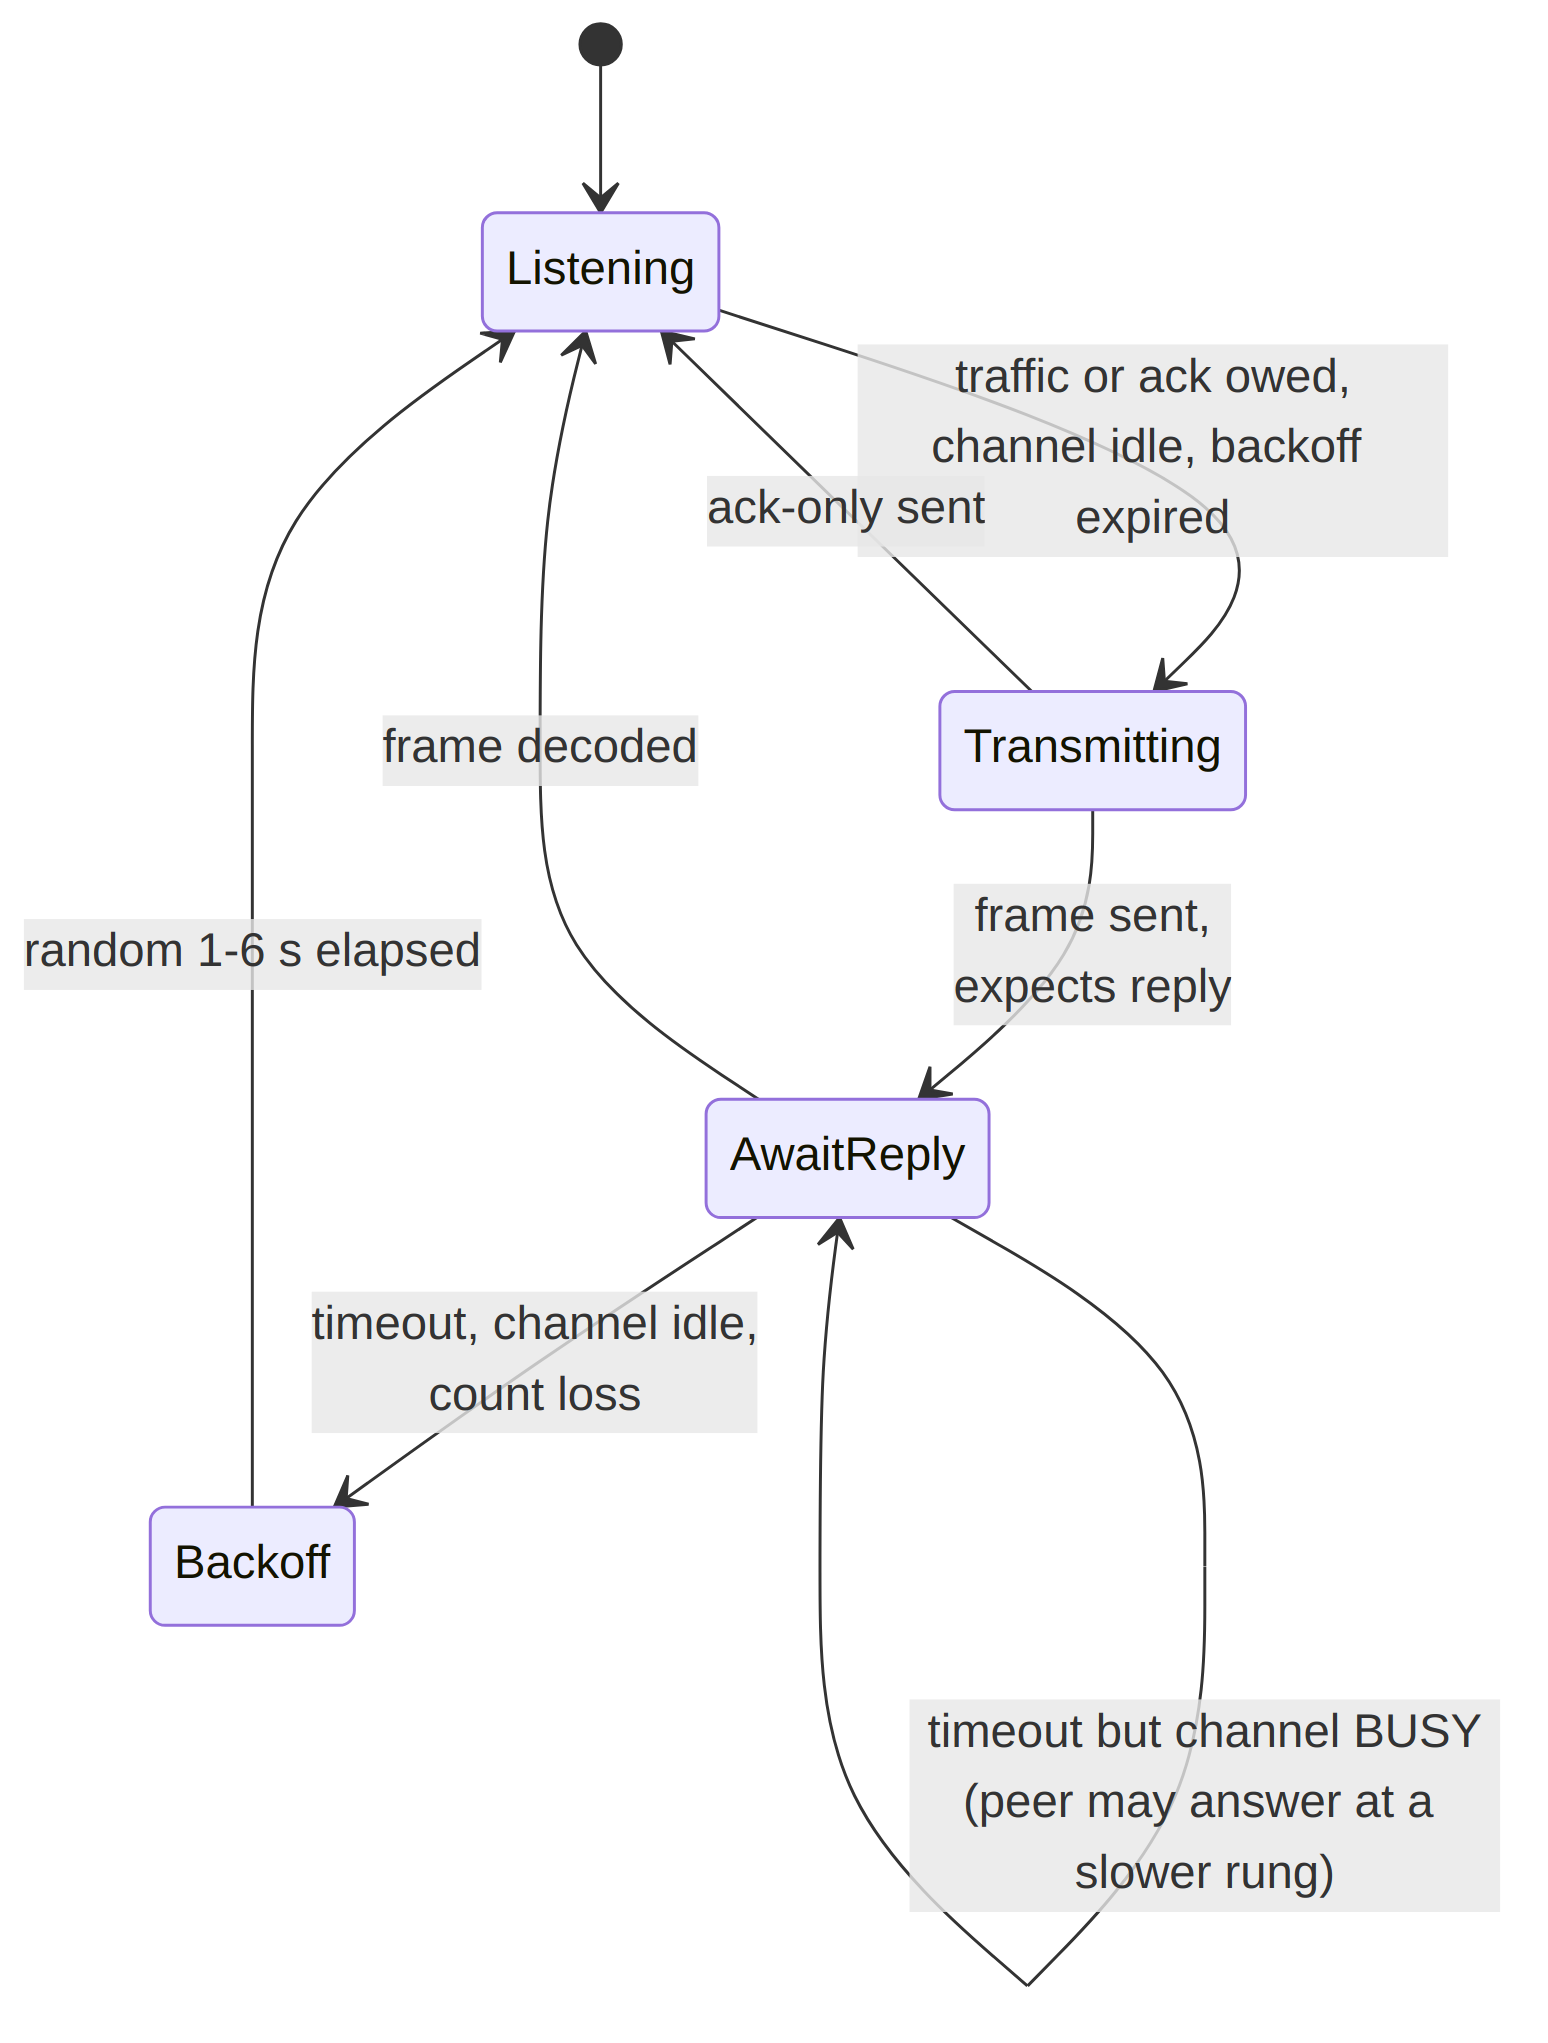
\includegraphics[width=0.85\textwidth]{images/simplex_state.png}
    \caption{Simplex channel-access state machine
             (\texttt{LinkStation.poll\_tx}).}
    \label{fig:simplex}
\end{figure}

The whole-system test (\texttt{experiments/simplex\_session.py}) runs
two stations with bidirectional QoS traffic and a $-14$\,dB fade in
the middle of the bulk transfer: all messages deliver bit-exact in QoS
priority order, the fade costs four timeouts and one
fallback-and-recover cycle, and the session terminates without
deadlock at 11--22\,bit/s effective on the shared channel.
Figure~\ref{fig:link_adaptation} shows the controller-level
simulation: bootstrap at EXTREME, a fast climb to the QPSK rungs,
loss-driven fallback within two frames of a sudden fade, and
recovery.

\begin{figure}[H]
    \centering
    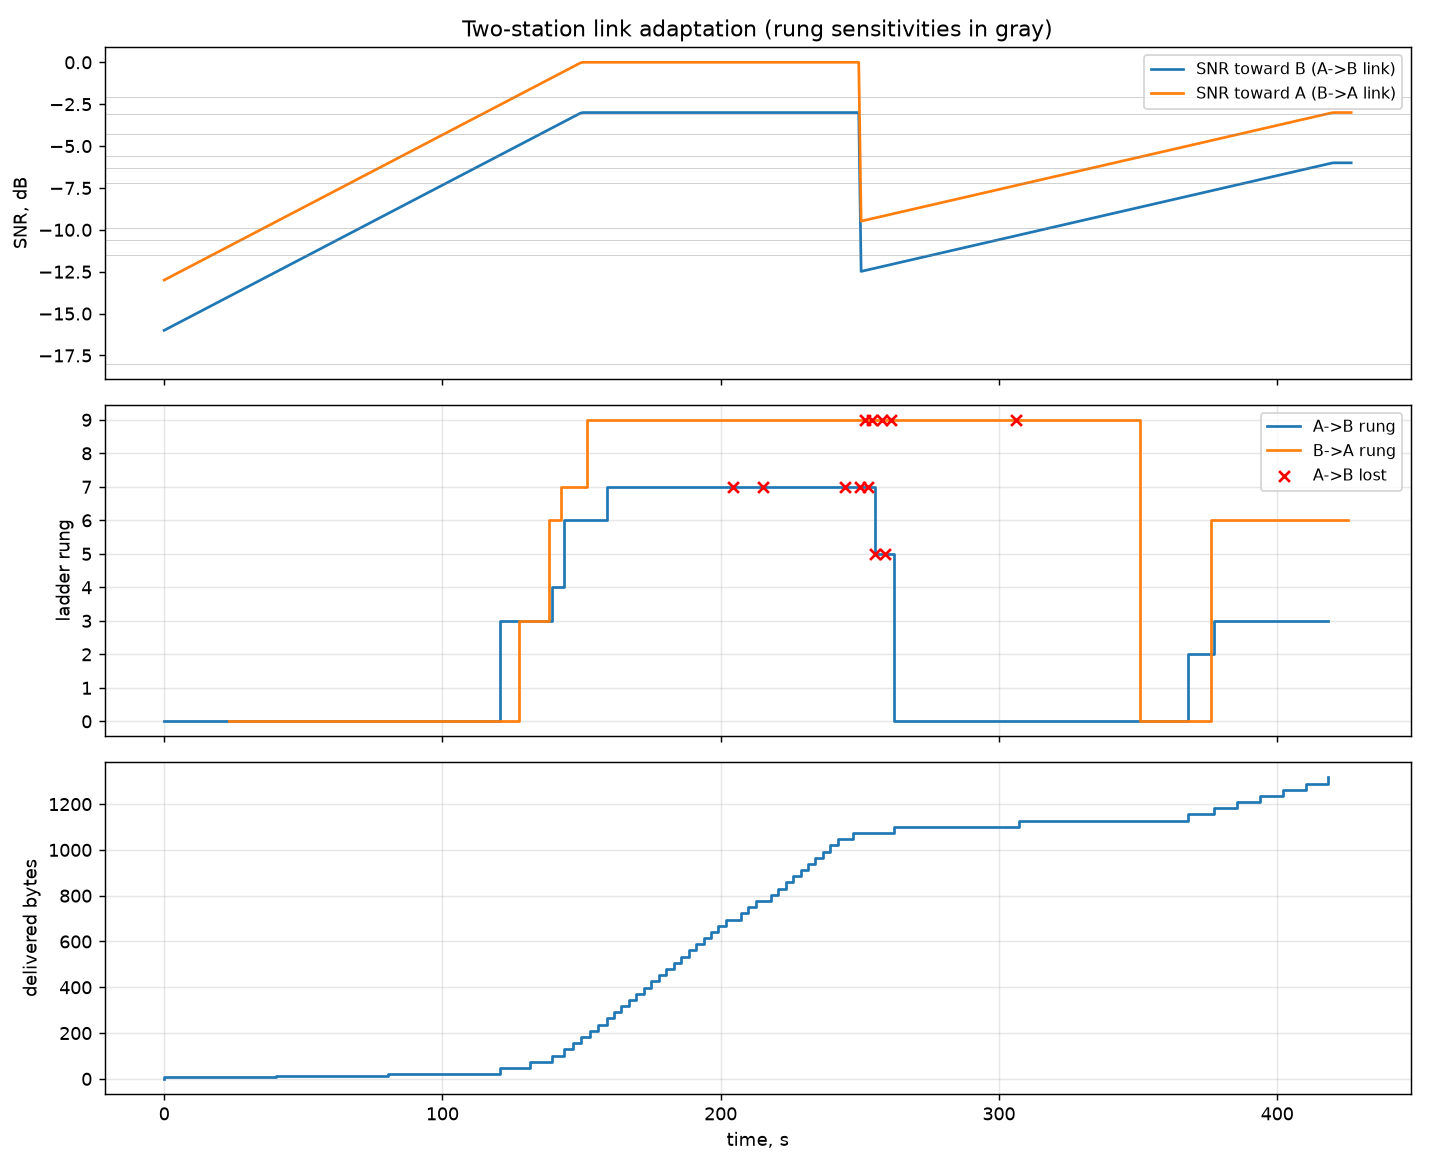
\includegraphics[width=\textwidth]{images/link_adaptation.png}
    \caption{Controller-level two-station simulation
             (\texttt{experiments/link\_adaptation.py}): asymmetric
             channel, $-16$\,dB start, sudden fade; 1290/1500 bytes
             delivered at 24\,bit/s effective goodput including ACK
             overhead and turnarounds.}
    \label{fig:link_adaptation}
\end{figure}

\subsection{The Capability Handshake, and 2\,kB Messages}
\label{sec:cport_caps}

The last structural inefficiency the two-board stand exposed was not a
defect but a shape. A 68\,kB file went out as 290 console parts, each
part one 256-byte station message, each message two burst fragments ---
so the link paid one acknowledgment per 260 bytes and reached about
50\,B/s at rung~12, on a wire whose raw rate is $\sim$1\,kbit/s. The
cap was \texttt{ST\_MSG\_MAX}: a message is one pool slot, and a
two-fragment transfer can never fill the eight-fragment window the
streaming machinery was built for. And underneath that sat a protocol
habit worth retiring: everything a station knew about its peer, it had
learned \emph{by failing at it}. Streaming capability was inferred from
a window that came back one-eighth acked
(Section~\ref{sec:burstwin}), then re-probed every eight transfers in
case the verdict was a forged fade; the fragment size was chosen from
the sender's own limits; and \texttt{sendfile} opened with a bare
\texttt{LINK} frame whose only job was to make the ladder move.

The handshake (Figure~\ref{fig:capsseq}) makes the peer's abilities
declared instead of discovered. A record --- version, capability bits
(\texttt{stream ext ldpc burst bcast}, later \texttt{bc\_stats}),
message size, window ceiling, pool slots, firmware version, and, from
the voice work of \S\ref{sec:voice_onair}, the maximum rung and a
codec bitmap: ten bytes when first built, eleven now, accepted from ten
because it grows without a version bump --- rides a Data frame
whose link-control flags are 7, the third combination impossible in
the legacy protocol (the burst frames took the other two). Three legs:
the initiator sends its record when it has bulk traffic and knows
nothing about the peer; the peer stores it and answers with its own
record plus an acknowledgment bit; the initiator's next frame carries
an ack of that sequence number, which is the third leg --- the peer
now knows its record arrived. On the stand the whole exchange costs
one second at the control rung:

\begin{quote}\ttfamily\small
23:05:23 [A] . caps sent: stream ext ldpc burst bcast  msg 2048 B, window 8\\
23:05:24 [A] . caps received: stream ext ldpc burst bcast  msg 2048 B, window 8
\end{quote}

\begin{figure}[htbp]
    \centering
    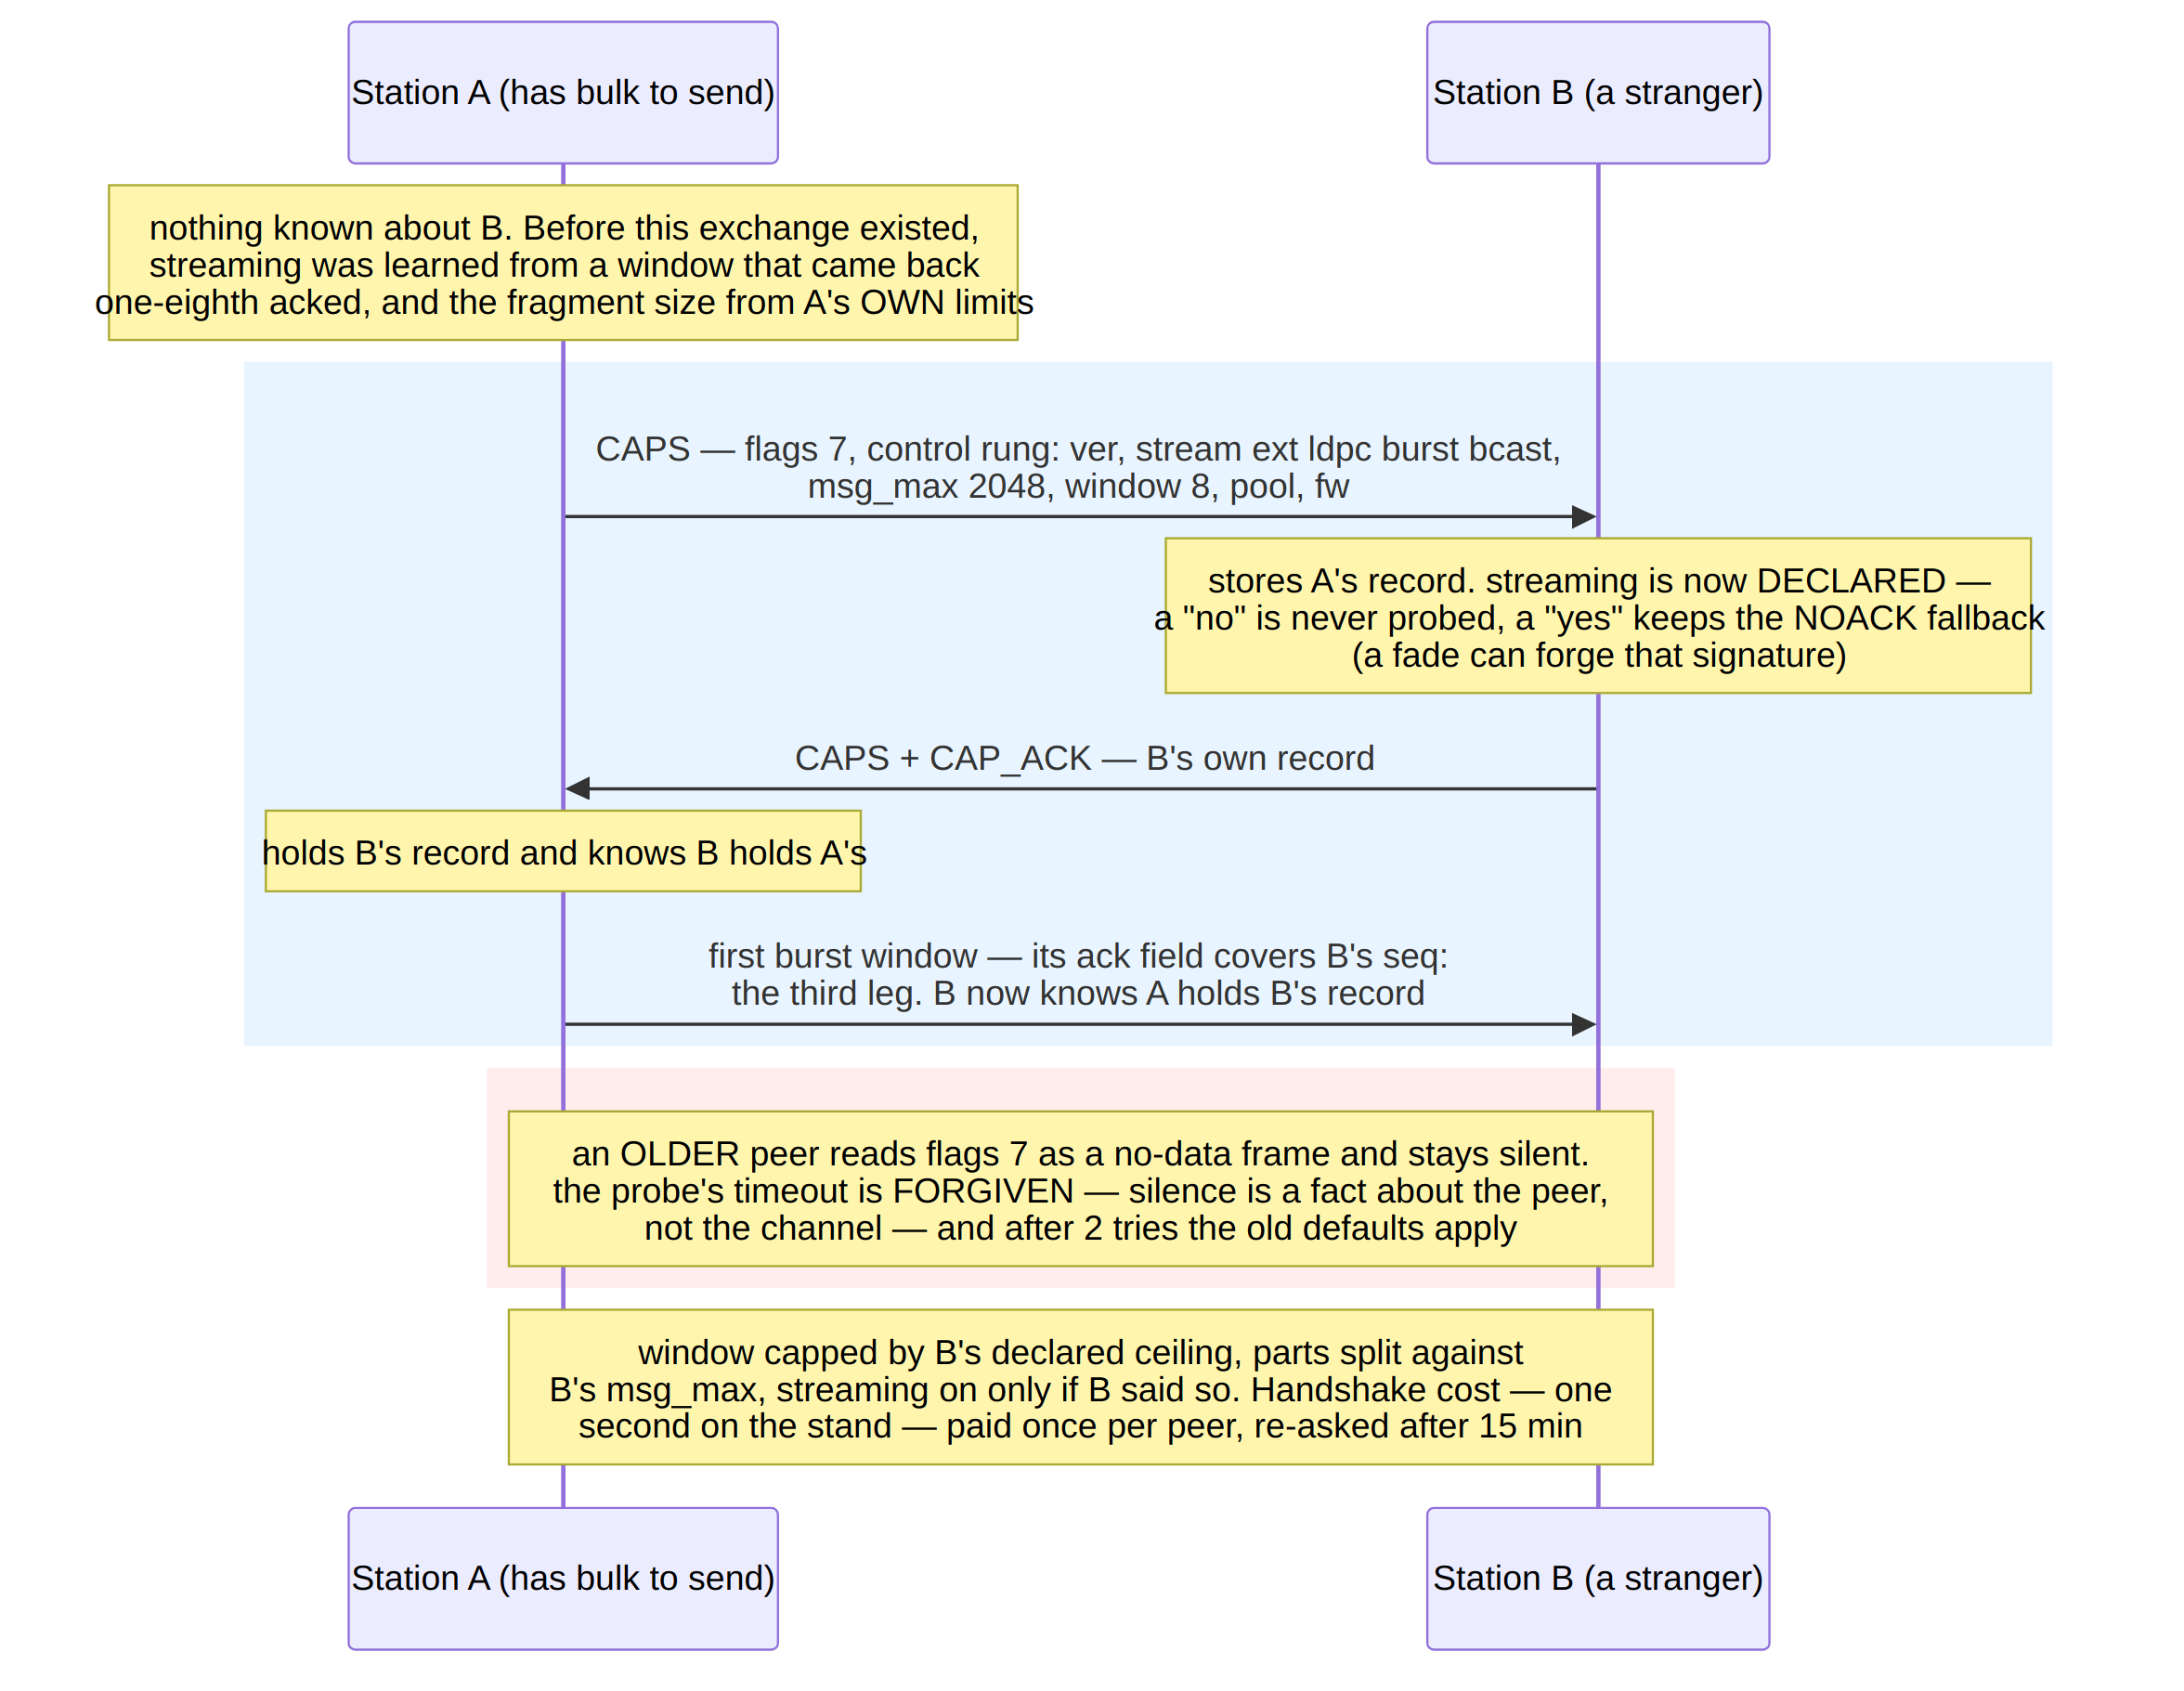
\includegraphics[width=0.82\textwidth]{images/caps_seq.png}
    \caption{The three-leg capability handshake. The record rides the
             third impossible flag combination, so an older peer reads
             it as a no-data frame and simply does not answer --- which
             is itself the answer, and is forgiven rather than charged
             to the rate controller.}
    \label{fig:capsseq}
\end{figure}

Three properties carried the design:

\paragraph{Silence is a fact about the peer, not the channel.} An
older firmware reads flags~7 as a no-data frame and never answers, so
the probe's timeout is \emph{forgiven} by the rate controller ---
charging it would walk \texttt{consecutive\_losses} toward the hard
rung-0 fallback for talking to an old radio --- and after two
unanswered tries the peer is marked legacy and today's defaults apply,
re-asked after five minutes. This is measured in the test suite: the
legacy-peer case completes its transfer on the defaults with the
ladder untouched.

\paragraph{A declaration outranks every inference.} A peer that says
it cannot stream is never streamed to --- the retry counter is set to a
value no clean exchange can reset, where the old NOACK verdict was
deliberately re-probed. A peer that says it \emph{can} keeps the NOACK
fallback anyway, because a deep fade can still forge the
one-fragment-acked signature and the channel remains entitled to its
opinion. And the declared streaming bit comes from the operator's
\texttt{burst\_stream} knob, \emph{not} from the PHY's
\texttt{receive\_burst} hook: the streaming receivers (demoapp and the
firmware) leave that hook NULL by design and walk streams through
\texttt{rxs\_continue\_burst}, and the first version --- which masked
the bit on the hook --- sent the smoke test from 5 frames to 29,
every window transmitted per-frame against a peer that streams
perfectly well.

\paragraph{The record's numbers are the receiver's, not the
sender's.} The window is capped at engage by the peer's declared
ceiling, and the consoles split files against the smaller of the two
message limits: the board reports its own \texttt{ST\_MSG\_MAX} in the
USB INFO reply and the peer's record in every status frame.

With the peer's limit known, the boards' limit could grow to meet it.
As a first step \texttt{ST\_MSG\_MAX} went to 2048 on the radio
firmware (the station moved wholesale to DTCM for the 21\,kB the pool
grew --- Section~\ref{sec:cport_memory}'s placement rules made that a
two-line change), and one USB frame carried one whole message; the
transfer measurements of \S\ref{sec:cport_levers} then took it to
the shipping 3328 bytes with the station in SRAM4. The same
68\,kB file became 34 parts of eleven fragments, each part one
streamed window:

\begin{center}
\begin{tabular}{lcc}
\hline
 & before & after \\
\hline
shape & 290 parts $\times$ 2 fragments & 34 parts $\times$ 8-fragment windows \\
acknowledgments & one per 260\,B & one per $\sim$1.6\,kB \\
transfer time & $\sim$25\,min & \textbf{13.0\,min, byte-exact} \\
\hline
\end{tabular}
\end{center}

The first full-size run also handed over one more calibration. Thirteen
of 34 windows timed out --- every one a forgiven first miss, so nothing
broke --- and the diagnostic stream showed why: after a 13.4-second
streamed window the receiver answers only after its end-of-stream
commit, which arrives as one $\sim$2.5\,s \texttt{rxs\_push}
(Section~\ref{sec:cport_radio} measured the stall) plus carrier
release. The reply timer's RFC-6298 smoothing had learned the
\emph{common} overhead --- 70\,ms, from the short exchanges --- and a
bimodal distribution is exactly what exponential smoothing cannot
hold. The stall is physics, not latency to learn, so it gets a fixed
allowance: a reply awaited after a streamed window adds
\texttt{RTO\_STREAM\_COMMIT\_S} (5\,s) to the budget, and streamed
exchanges no longer feed the estimator at all. The re-run: 4 timeouts
instead of 13, zero retransmissions, and the same 780-second
transfer time --- the allowance only lengthens waits for acks that are
late anyway.

\subsubsection{The ceilings become operator knobs}

The record's window field had been the compile-time buffer limit, and
the protocol had carried a related embarrassment since its first
revision: \texttt{config rung\_ceiling} --- the operator's cap on the
rate ladder --- was documented in the USB key list and implemented
nowhere. The modem's configuration handler simply had no case for it,
and nothing ever noticed, because nothing ever read the setting.

Both ceilings are now real, runtime, and declared. \texttt{config
win\_max} bounds the streamed window this station accepts \emph{and}
sends (byte 4 of the record); \texttt{config rung\_ceiling} bounds
the rung it transmits at or requests (byte 9, encoded as
ceiling$+$1 so the zero an older firmware sends still reads as
``unspecified''). Changing either while a peer is known pushes a
refreshed record at once, rather than waiting for the next transfer to
re-handshake.

Enforcement sits in the station, deliberately outside the rate
controller: every transmit-rung decision passes through a clamp ---
the controller's choice, bounded by our own ceiling and by the fastest
rung the peer declared --- because clamping \emph{inside} the
controller would poison its per-rung offset learning with rungs it
never actually chose. Requests are clamped the same way, and the
window at engage is the minimum of the operator window, the buffer
limit, our declared ceiling and the peer's.

The verification ran over USB, no rebuild involved: board~B was given
\texttt{win\_max 4} and \texttt{rung\_ceiling 9} from its console,
and board~A --- whose controller wanted rung~12 on a clean wire ---
sent fourteen frames at rung~9 and none above, every window engage
reading \texttt{4 of 16 (ceiling)}, with A's status line showing the
declared limits: \texttt{window 4, rung ceiling 9 (handshake
complete)}. The suite holds the same case synthetically: a peer
declaring window~4 and ceiling~9 against a controller that wants the
top rung, asserted on both the window and every frame's rung.

\subsection{AFC Frequency Netting}
\label{sec:afc}

The receiver measures the peer's carrier offset on every decoded frame
anyway (\texttt{stats.cfo\_hz}), so the link closes the loop: the
5-bit LC field carries ``shift your carrier by $-X$\,Hz'' requests
($\pm 120$\,Hz per frame, 8\,Hz steps, $\pm 12$\,Hz deadband), and the
peer trims its \emph{shared} reference oscillator.  Trimming the
shared reference moves TX and RX together --- which is exactly why
asking the peer to correct beats retuning locally
(Section~\ref{sec:rf}).  Corrections are applied at \textbf{half
gain}: both sides act on measurements that are one frame stale, and
full-gain corrections would swap the offset between the stations each
turn instead of converging (Figure~\ref{fig:afc}).

\begin{figure}[H]
    \centering
    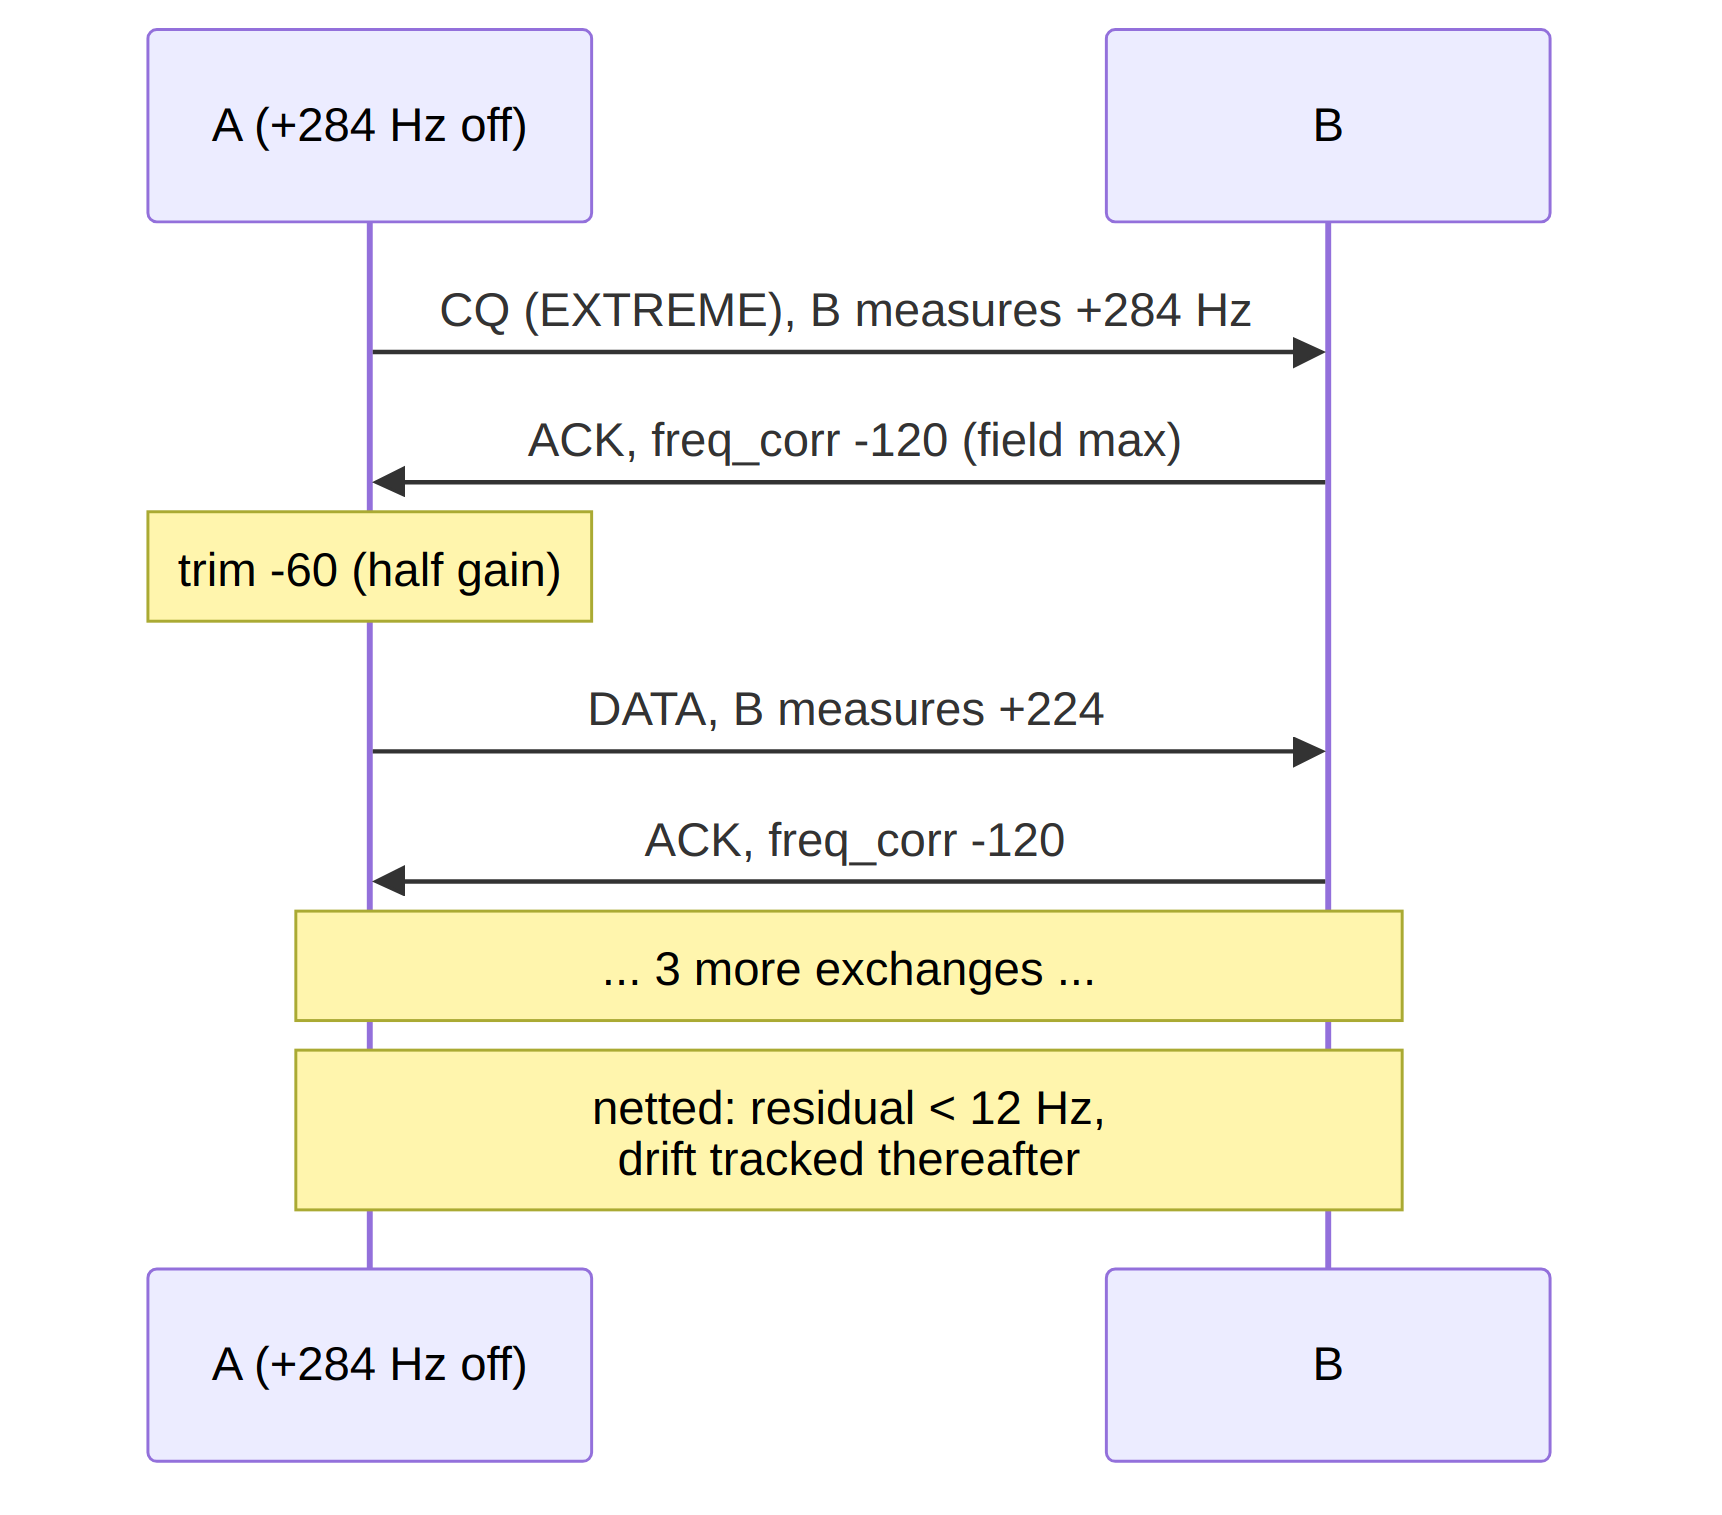
\includegraphics[width=0.85\textwidth]{images/afc_seq.png}
    \caption{AFC netting from a $+284$\,Hz initial offset.}
    \label{fig:afc}
\end{figure}

\subsubsection{Guard Rails}

The loop observes only the \emph{differential} offset, so without
bounds the pair's common frequency random-walks over a long session
--- out of the channel slot, into bystanders' passbands, or off the
rig's trim range.  Two mechanisms bound it:

\begin{itemize}
    \item \texttt{afc\_max\_trim\_hz} (default $\pm 150$\,Hz)
          hard-clamps each station's \emph{cumulative} trim.  Requests
          beyond the budget are partially honoured or refused, the
          peer's own headroom carries the rest, and any residual is
          left to the modem's $\pm 300$\,Hz CFO tolerance --- the link
          keeps working, just without full netting.
    \item \texttt{afc\_anchor=True} designates a station (e.g.\ the CQ
          caller) that never trims, pinning the absolute frequency
          entirely; the peer does all the correcting.
\end{itemize}

\subsubsection{Measured Behaviour}

\texttt{experiments/afc\_netting.py} runs two worn-TCXO rigs on
14.2\,MHz starting \textbf{$+284$\,Hz apart} (near the modem's
$\pm 375$\,Hz limit) with opposing thermal drifts: netted to within
the deadband in $\approx$5 correction exchanges ($\approx$104\,s ---
EXTREME bootstrap frames dominate the wall clock), steady-state
$|$CFO$| \le 11$\,Hz under continuing 0.09\,Hz/s relative drift,
400/400 bytes delivered.  The guard scenarios behave as designed:
default budgets net fully (final $|$CFO$|$ 3\,Hz, trims clamped at
$-150/+144$\,Hz); deliberately tight $\pm 40$\,Hz budgets stop at
their limits leaving a 222\,Hz residual \emph{by design}, with the
link still delivering on CFO tolerance alone; an anchored station A
forces B to absorb the full $+292$\,Hz and the pair's absolute
frequency never moves.  Beyond robustness margin, a netted link could
shrink EXTREME's per-symbol frequency-search range (compute) and eases
mask-grid detection at the extremes.
